\chapter{Реализация прототипа плагина} \label{ch3}

% не рекомендуется использовать отдельную section <<введение>> после лета 2020 года
%\section{Введение. Сложносоставное название первого параграфа первой главы для~демонстрации переноса слов в содержании} \label{ch1:intro}
В 3 главе будут рассмотрены и описаны основные классы, которые были разработаны в соответствии с диаграммой классов из приложения 1, а также полученные результаты.

\section{Описание разработанных классов} \label{ch3:sec1}

В процессе написания кода плагины были запрограммированы классы в соответствии с диаграммой классов из приложения 1.

\subsection{BuildConfigurationStatisticsAction}

Основной класс приложения, который реализует интерфейс действия, через этот класс происходит взаимодействие с Jelly, а также вызов всех остальных методов бизнес-логики плагина, и определены поля для работы со сборками, все методы для получения информации о конкретной метрике сборки помечены аннотацией @JavaScript для того, чтобы можно было их вызывать через JS в Jelly, также во всех этих методах тип возвращаемого объекта приведен к JSON, который и передается в DOM страницы плагина при взаимодействии с элементами пользовательского интерфейса.

В классе реализованы только одно закрытое поле job, с помощью которого происходит взаимодействие со сборкой в проекте, а также обработка выполненных запусков. А также следующие методы:

\begin{itemize}
	\item BuildConfigurationStatisticsAction(Job job) - конструктор класса;
	\item String getIconFileName() - метод, определяющий иконку приложения в боковом меню;
	\item String getDisplayName() - метод, определяющий отображаемое имя плагина в боковом меню и других частях страницы;
	\item String getUrlName() - метод, определяющий url, по которому доступна страница плагина;
	\item Job getJob() - метод-геттер для получения текущей сборки;
	\item String getBuildDuration(String period, String fail, String statistics) - метод для получения информации о времени продолжительности запусков сборки, за определенный период, с заданными настройками;
	\item String getBuildSuccessRate(String period) - метод для получения информации о проценте успешности выполнения запусков сборки, за определенный период;
	\item String getBuildArtifactSize(String period, String fail, String statistics) - метод для получения информации о созданных артефактов запусков сборки, за определенный период, с заданными настройками;
	\item String getBuildTestCount(String period, String fail) - метод для получения информации о количестве выполненных тестов при запуске сборки, за определенный период, с заданными настройками;
	\item String getBuildTimeQueue(String period, String statistics) - метод для получения информации о времени нахождения в очереди запусков сборки, за определенный период, с заданными настройками.
\end{itemize}

\subsection{DateTimeHandler}

Статический класс, созданный для взаимодействия с датами и их обработки при создании структур данных, которые также создаются в рамках этого класса, формирования структуры данных зависит от метрики и от периода за который нужно получить информацию.

В классе определено поле Logger LOGGER, с помощью которого записываются логи плагина. Также в классе определены методы:

\begin{itemize}
	\item Date convertLongTimeToDate(long time) - метод, преобразующей время в миллисекундах, прошедших с 1970 года, в дату типа Date;
	\item long convertDateToLongTime(Date date) - метод, преобразующей дату в миллисекунды, прошедшие с 1970 года;
	\item int getDayOfMonth(Date aDate) - метод, получающий номер дня из даты в месяце;
	\item int getLastMonthDays() - метод для получения дней в прошлом месяце;
	\item String dateToString(Date date, String format) - метод для преобразования типа Date, в строку в соответствии с заданным форматом даты;
	\item String dateMonthToString(Date date) - метод для преобразования типа Date, в строку в соответствии с форматом "yyyy-MM";
	\item String dateSetZeroMinutesSeconds(String dateString) - метод для обнуления минут и секунд в строке с датой;
	\item HashMap<String, List<Double>> createDateMonthMap() - метод, создающий начальную структуру данных за прошедший месяц по дням, где в качестве значений словаря используются пустые списки;
	\item HashMap<String, List<Double>> createDateAllMap(RunList<Run> runs) - метод для создания начальной структуры данных, за весь прошедший период, который вычисляет на какие равные интервалы следует разбить общий промежуток времени, от создания первой сборки, до создания последней сборки;
	\item HashMap<String, List<Double>> createDateDayMap() - метод, создающий начальную структуру данных за прошедший день по часам, где в качестве значений словаря используются пустые списки;
	\item HashMap<String, HashMap<String,Integer>> createDateDayMapSuccess() - метод, создающий начальную структуру данных за прошедший день по часам, для вычисления процента успешности выполнения сборок, где в качестве значений словаря используется словарь, в котором записано сколько запусков сборки выполнено успешно, а сколько с ошибками;
	\item HashMap<String, HashMap<String,Integer>> createDateWeekMapSuccessRate() - метод, создающий начальную структуру данных за прошедшую неделю по дням, для вычисления процента успешности выполнения сборок, где в качестве значений словаря используется словарь, в котором записано сколько запусков сборки выполнено успешно, а сколько с ошибками;
	\item HashMap<String, HashMap<String,Integer>> createDateMonthMapSuccessRate() - метод, создающий начальную структуру данных за прошедший месяц по дням, для вычисления процента успешности выполнения сборок, где в качестве значений словаря используется словарь, в котором записано сколько запусков сборки выполнено успешно, а сколько с ошибками;
	\item HashMap<String, HashMap<String,Integer>> createDateQuarterMapSuccessRate() - метод, создающий начальную структуру данных за прошедший квартал по месяцам, для вычисления процента успешности выполнения сборок, где в качестве значений словаря используется словарь, в котором записано сколько запусков сборки выполнено успешно, а сколько с ошибками;
	\item HashMap<String, Integer> createDateMonthMapTestCount() - метод, создающий начальную структуру данных за прошедший месяц по дням, для вычисления количества выполненных тестов во время запуска сборки, где в качестве значений словаря используется целочисленные нули;
	\item HashMap<String, Integer> createDateDayMapTestCount() - метод, создающий начальную структуру данных за прошедший день по часам, для вычисления количества выполненных тестов во время запуска сборки, где в качестве значений словаря используется целочисленные нули;
	\item HashMap<String, Integer> createDateYearMapTestCount() - метод, создающий начальную структуру данных за прошедший год по месяцам, для вычисления количества выполненных тестов во время запуска сборки, где в качестве значений словаря используется целочисленные нули;
	\item HashMap<String, Integer> createDateQuarterMapTestCount() - метод, создающий начальную структуру данных за прошедший квартал по месяцам, для вычисления количества выполненных тестов во время запуска сборки, где в качестве значений словаря используется целочисленные нули;
	\item HashMap<String, Integer> createDateWeekMapTestCount() - метод, создающий начальную структуру данных за прошедшую неделю по дням, для вычисления количества выполненных тестов во время запуска сборки, где в качестве значений словаря используется целочисленные нули;
	\item HashMap<String, List<Double>> createDateYearMap() - метод, создающий начальную структуру данных за прошедший год по месяцам, где в качестве значений словаря используются пустые списки;
	\item HashMap<String, List<Double>> createDateQuarterMap() - метод, создающий начальную структуру данных за прошедший квартал по месяцам, где в качестве значений словаря используются пустые списки;
	\item HashMap<String, List<Double>> createDateWeekMap() - метод, создающий начальную структуру данных за прошедшую неделю по дням, где в качестве значений словаря используются пустые списки;
	\item HashMap<String, HashMap<String,Integer>> createDateYearMapSuccessRate() - метод, создающий начальную структуру данных за прошедший год по месяцам, для вычисления процента успешности выполнения сборок, где в качестве значений словаря используется словарь, в котором записано сколько запусков сборки выполнено успешно, а сколько с ошибками.
\end{itemize}
	
	\subsection{IntervalDate}
	
	Перечисляемый тип для удобства работы с датами-периодами. Содержит следующие предопределенные константы:
	
	\begin{itemize}
	\item DAY - день;
	\item WEEK - неделя;
	\item MONTH - месяц;
	\item YEAR - год;
	\item QUARTER - квартал;
	\item ALL - константа для определения, того что будут вычисляться равные периоды для данных за все время, от начального запуска сборки до конечного.
\end{itemize}

	\subsection{Statistics}
	
	Перечисляемый тип для удобства работы с показателями статистики. Содержит следующие предопределенные константы:
	
	\begin{itemize}
	\item SUM - сумма;
	\item AVG - среднее;
	\item MEDIAN - медиана;
	\item RANGE - размах;
	\item DISPERSION - дисперсия;
	\item SDUNBIASED - среднеквадратичное отклонение несмещенное;
	\item MODE - мода;
	\item SD - среднеквадратичное отклонение.
\end{itemize}

\subsection{TimeInQueueFetcher}

Класс отвечающий за расчет времени, которая сборка провела в очереди перед тем как отправилась на выполнение. В классе определен один метод long getTimeInQueue(Run build) с помощью которого вычисляется нахождение времени в очереди в миллисекундах для конкретного запуска сборки.

\subsection{BuildLogic}
	
Базовый класс бизнес-логики, от которого наследуются все остальные более специфичные классы по каждой метрике, в классе определяются методы фильтрации по периоду и наличию упавших сборок в итоговых результатах. В классе определены следующие поля:

\begin{itemize}
	\item IntervalDate period - период за который производится отбор запусков сборок для дальнейшей обработки и визуализации;
	\item RunList<Run> buildList - список запусков у конкретной сборки;
	\item Boolean failed - поле, которое определяет нужно ли учитывать при обработке и визуализации упавшие сборки (true - надо учитывать);
	\item Logger LOGGER - поле, с помощью которого записываются логи плагина при выполнении методов класса.
\end{itemize}

Также в классе определены методы, которые наследуются всеми остальными классами бизнес-логики, которые отвечают за работу с определенной метрикой:

\begin{itemize}
	\item BuildLogic(IntervalDate period, Boolean failed, RunList<Run> buildList) - конструктор класса;
	\item void filterPeriodBuild() - метод, который производит отборок только тех запусков, которые удовлетворяют заданному периоду;
	\item void filterFailedBuild() - метод, который производит отборок только тех запусков, которые удовлетворяют полю failed, т.е. в зависимости от значения флага, либо включает в выборку упавшие сборки, либо нет.
\end{itemize}

\subsection{BuildArtifactSizeLogic}

Класс для работы с метрикой AS, в нем происходит пересчет параметров в зависимости от периода и настроек подданных на вход, а также высчитывается размер артефакта в Кб. В классе определены следующие поля:

\begin{itemize}
	\item HashMap<String, Double> dateFormatArtifact - структура данных для работы с запусками сборки относительно метрики AS, ключи даты за выбранный период, значения размер артефактов, созданных во время запуска за выбранный период;
	\item String dateFormatKey - поле, которое определяет формат даты за выбранный период, по которому будет происходить обработка и визуализация;
	\item Logger LOGGER - поле, с помощью которого записываются логи плагина при выполнении методов класса.
\end{itemize}

Также в классе определены методы:

\begin{itemize}
	\item BuildArtifactSizeLogic(IntervalDate period, Boolean failed, RunList<Run> buildList) - конструктор класса;
	\item Map<String, Double> getArtifactSize(Statistics statistics) - метод, в котором происходит фильтрация данных запусков сборок по периоду и флагу failed, определение формата дат и вычисление размера артефактов в Кб, а также расчет по статистической величине (например, среднее арифметическое), в зависимости от заданных настроек.
\end{itemize}

\subsection{BuildDurationLogic}

Класс для работы с метрикой BD, в нем происходит пересчет параметров в зависимости от периода и настроек подданных на вход, а также высчитывается продолжительность сборки в секундах. В классе определены следующие поля:

\begin{itemize}
	\item HashMap<String, Double> dateFormatDuration - структура данных для работы с запусками сборки относительно метрики BD, ключи даты за выбранный период, значения время выполнения запусков сборки за выбранный период;
	\item String dateFormatKey - поле, которое определяет формат даты за выбранный период, по которому будет происходить обработка и визуализация;
	\item Logger LOGGER - поле, с помощью которого записываются логи плагина при выполнении методов класса.
\end{itemize}

Также в классе определены методы:

\begin{itemize}
	\item BuildDurationLogic(IntervalDate period, Boolean failed, RunList<Run> buildList) - конструктор класса;
	\item Map<String, Double> getBuildsDuration(Statistics statistics) - метод, в котором происходит фильтрация данных запусков сборок по периоду и флагу failed, определение формата дат и вычисление времени выполнения запусков сборок, а также расчет по статистической величине (например, среднее арифметическое), в зависимости от заданных настроек.
\end{itemize}

\subsection{BuildSuccessRateLogic}

Класс для работы с метрикой SR, в нем происходит пересчет параметров в зависимости от периода, а также высчитывается процент успешности выполненных сборок за заданный промежуток времени. В классе определены следующие поля:

\begin{itemize}
	\item HashMap<String, HashMap<String,Integer>> successRateOnFormatDate - структура данных для работы с запусками сборки относительно метрики SR, ключи даты за выбранный период, значения процент успешности выполнения запусков сборки за выбранный период;
	\item String dateFormatKey - поле, которое определяет формат даты за выбранный период, по которому будет происходить обработка и визуализация;
	\item Logger LOGGER - поле, с помощью которого записываются логи плагина при выполнении методов класса.
\end{itemize}

Также в классе определены методы:

\begin{itemize}
	\item BuildSuccessRateLogic(IntervalDate period, RunList<Run> buildList) - конструктор класса;
	\item Map<String, Double> getSuccessRate() - метод, в котором происходит фильтрация данных запусков сборок по периоду, определение формата дат и вычисление процента успешности выполнения запусков сборок.
\end{itemize}

\subsection{BuildTestCountLogic}

Класс для работы с метрикой TS, в нем происходит пересчет параметров в зависимости от периода и настроек подданных на вход, а также высчитывается количество выполненных тестов во время работы сборок за определенный период. В классе определены следующие поля:

\begin{itemize}
	\item HashMap<String, Integer> testCountOnFormatDate - структура данных для работы с запусками сборки относительно метрики TC, ключи даты за выбранный период, значения количество выполненных тестов запусков сборки за выбранный период;
	\item String dateFormatKey - поле, которое определяет формат даты за выбранный период, по которому будет происходить обработка и визуализация;
	\item Logger LOGGER - поле, с помощью которого записываются логи плагина при выполнении методов класса.
\end{itemize}

Также в классе определены методы:

\begin{itemize}
	\item BuildTestCountLogic(IntervalDate period, RunList<Run> buildList) - конструктор класса;
	\item Map<String, Integer> getTestCount() - метод, в котором происходит фильтрация данных запусков сборок по периоду и флагу failed, определение формата дат и вычисление количества выполненных тестов в процессе исполнения запусков сборки.
\end{itemize}

\subsection{BuildTimeQueueLogic}

Класс для работы с метрикой TQ, в нем происходит пересчет параметров в зависимости от периода и настроек подданных на вход, а также высчитывается время ожидание сборки в очереди в миллисекундах. В классе определены следующие поля:

\begin{itemize}
	\item HashMap<String, Double> dateFormatDuration - структура данных для работы с запусками сборки относительно метрики TQ, ключи даты за выбранный период, значения время нахождения в очереди запусков сборки за выбранный период;
	\item String dateFormatKey - поле, которое определяет формат даты за выбранный период, по которому будет происходить обработка и визуализация;
	\item Logger LOGGER - поле, с помощью которого записываются логи плагина при выполнении методов класса.
\end{itemize}

Также в классе определены методы:

\begin{itemize}
	\item BuildTimeQueueLogic(IntervalDate period, RunList<Run> buildList) - конструктор класса;
	\item Map<String, Double> getTimeQueue(Statistics statistics) - метод, в котором происходит фильтрация данных запусков сборок по периоду и флагу failed, определение формата дат и вычисление времени нахождения в очереди запусков сборок, а также расчет по статистической величине (например, среднее арифметическое), в зависимости от заданных настроек.
\end{itemize}

\subsection{Файлы JS и Jelly}

В JS определяются функции событий для выбора элемента из выпадающего списка и взаимодействия с флажками. Для каждой метрики используется своя функции, внутри определяются настройки данных и отображения для визуализации отдельной метрики в виде определенного графика/диаграммы, вызывается метод для сортировки агрегированных по датам значений метрик в структуре JSON, а также формируются метки-подписи для каждого типа периода.

Также в JS определены следующие функции:

\begin{itemize}
	\item formatLabelsDate(arrLabels, dateFormat, period) - функция, в которой происходит формирование меток-подписей к графикам в зависимости от формата дат и выбранного периода;
	\item sortOnKeys(dict, period) - функция в которой происходит сортировка значений словаря с данными о запусках сборок по ключам-датам;
	\item createSuccessRateChart() - функция в которой происходит подготовка данных, формирование настроек и создание графика по метрике SR;
	\item typeChartHandler(typeChart, labels, title, dictValues) - функция, которая обрабатывает событие изменение типа графика/диаграммы, и обновляет представление на странице плагина;
	\item createTestCountChart() - функция в которой происходит подготовка данных, формирование настроек и создание графика по метрике TC;
	\item createBuildDurationChart() - функция в которой происходит подготовка данных, формирование настроек и создание графика по метрике BD;
	\item createArtifactSizeChart() - функция в которой происходит подготовка данных, формирование настроек и создание графика по метрике AS;
	\item createTimeQueueChart() - функция в которой происходит подготовка данных, формирование настроек и создание графика по метрике TQ.
\end{itemize}

В jelly файле с помощью html формируется структура документа, а также выполняется привязка Java объектов к объектам JS. Определяются обработчики событий, который при взаимодействии с пользователем вызывают определенный запрос-метод AJAX.

\section{Результаты разработки плагина} \label{ch3:sec2}

При разработке плагина надо было учитывать, что требуется отображать все графики на одной странице задания друг под другом, поскольку при выборе одно периода, например, месяца, будет получена сводная информация по каждой сборке или нескольких сборок запущенных в один день. Графики отображаются посредством переходна на соответствующую ссылку, оставляя при этом пользователя в том же задании (странице с результатами последних сборок).

В интерфейсе у каждого графика были реализованы те дополнительные функции отображения, которые могут быть применены к визуализируемой метрике: отобразить статистику по упавшим сборкам/тестам, обработать метрику в соответствии со статистическим показателем.

Интерфейс страницы плагина с графиками в системе Jenkins на странице задания показан на рисунке 3.1.


\begin{figure}[ht!] 
	\center
	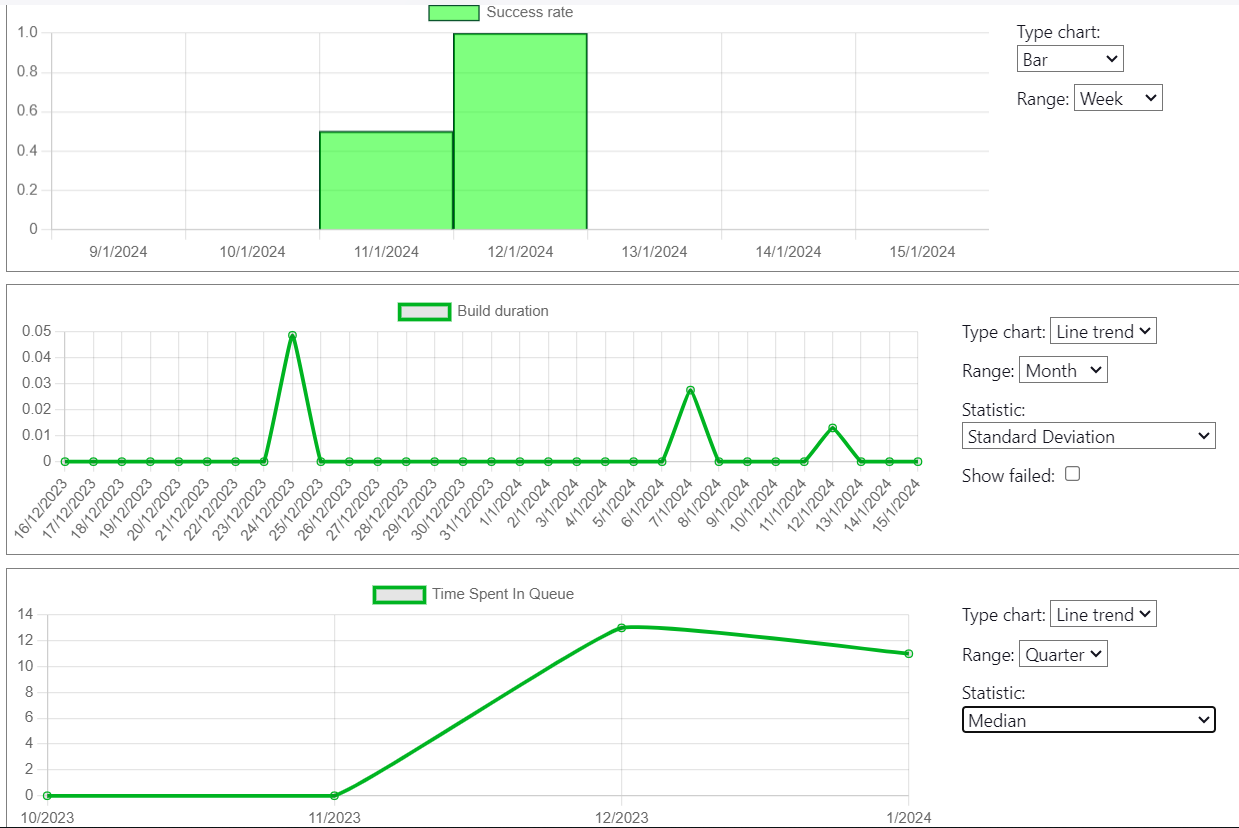
\includegraphics [scale=0.47] {my_folder/images//ui12}
	\caption{Интерфейс плагина Jenkins} 
	\label{fig:ui1}  
\end{figure}

Интерфейс страницы плагина в системе Jenkins с графиком AS на странице задания при выборе типа графика Radar, за период месяц, обработанные по показателю среднее арифметическое и учитывающий упавшие сборки представлен на рисунке 3.2.

\begin{figure}[ht!] 
	\center
	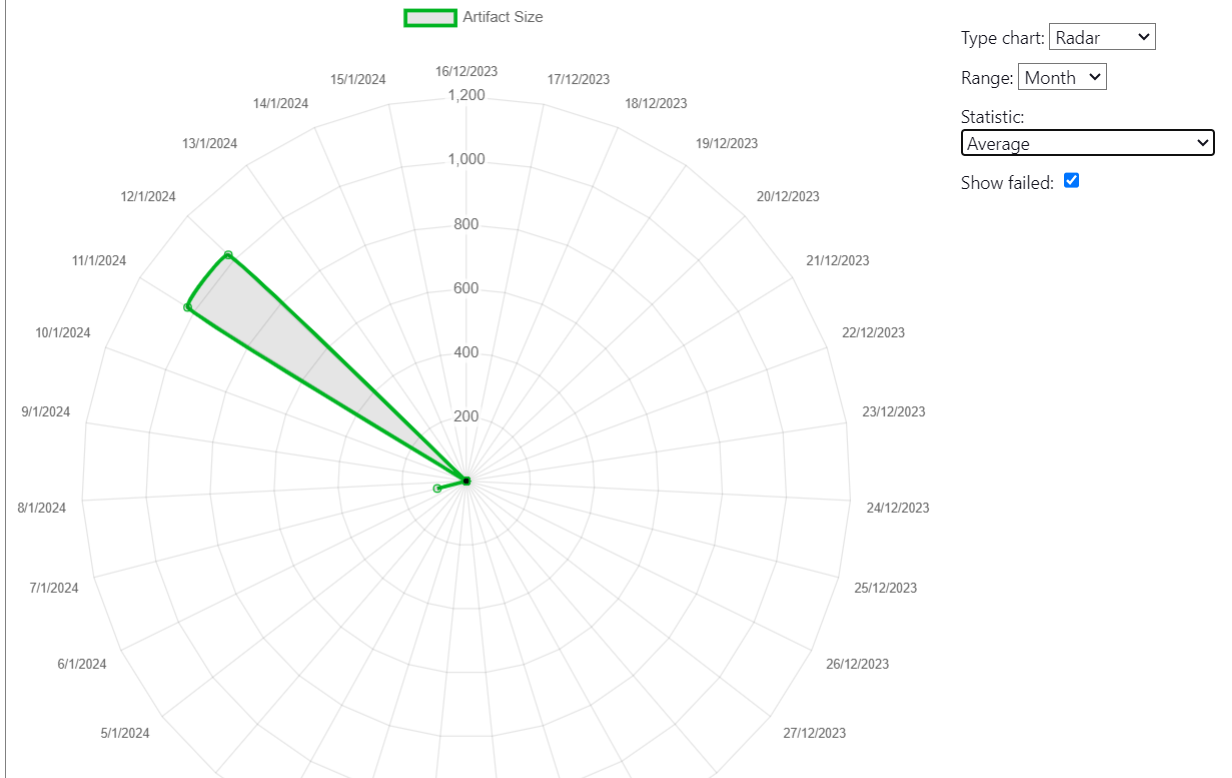
\includegraphics [scale=0.47] {my_folder/images//ui22}
	\caption{Интерфейс графика Radar для AS} 
	\label{fig:ui22}  
\end{figure}

Основное взаимодействие с графиками будет производить через меню, которое есть напротив каждого графика со своими параметрами, отображенном на рисунке 3.3:

\begin{figure}[ht!] 
	\center
	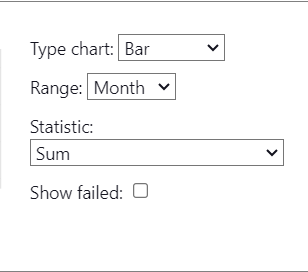
\includegraphics [scale=0.47] {my_folder/images//ui13}
	\caption{Интерфейс элементов управления} 
	\label{fig:ui13}  
\end{figure}

При взаимодействии с раскрывающимся списком должен вызываться Java метод, который пересчитает и отфильтрует необходимые сборки Jenkins и динамически отобразит результаты по выбранными периоду, также динамически должна производить обработка метрик сборок, при выборе статистического показателя, а также включение в графики данных об упавших сборках, при выборе соответствующих чекбоксов.

Интерфейс изменения навигационной панели отображен на рисунке 3.4. В данном случае видно что изменения видны при открытии конфигурации конкретной сборки, т.е. не надо будет переключаться между окном плагина и сборкой для визуализации метрик, при открытии данного пункта меню, также происходит изменения URL, с которым в дальнейшем и происходит взаимодействие.

\begin{figure}[ht!] 
	\center
	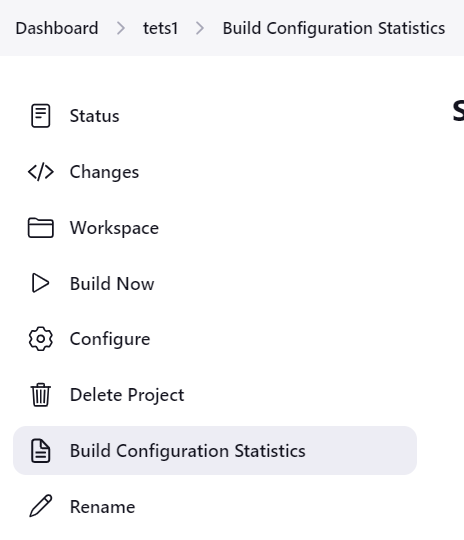
\includegraphics [scale=0.47] {my_folder/images//ui3}
	\caption{Интерфейс элементов управления} 
	\label{fig:ui3}  
\end{figure}


Код плагина представлен в приложении 4.
 
\section{Выводы} \label{ch3:sec3}

В главе 3 была проведена реализация плагина, а также описаны классы, разработанные при написании плагина и файлы, которые участвуют во взаимодействии с этими классами и отображаемым интерфейсом пользователя. Также были приведены результаты разработки, приведены скриншоты интерфейсов, а также описаны добавленные на страницу Jenkins элементы, после установки плагина.





%
%

%
%
%\begin{table} [htbp]% Пример оформления таблицы
%	\centering\small
%	\caption{Представление данных для сквозного примера по ВКР \cite{Peskov2004}}%
%	\label{tab:ToyCompare}		
%		\begin{tabular}{|l|l|l|l|l|l|}
%			\hline
%			$G$&$m_1$&$m_2$&$m_3$&$m_4$&$K$\\
%			\hline
%			$g_1$&0&1&1&0&1\\ \hline
%			$g_2$&1&2&0&1&1\\ \hline
%			$g_3$&0&1&0&1&1\\ \hline
%			$g_4$&1&2&1&0&2\\ \hline
%			$g_5$&1&1&0&1&2\\ \hline
%			$g_6$&1&1&1&2&2\\ \hline		
%		\end{tabular}	
%	\normalsize% возвращаем шрифт к нормальному
%\end{table}


% \firef{} от figure reference
% \taref{} от table reference
% \eqref{} от equation reference




